\artigotrue
\chapter{OPTIMIZATION OF SAMPLE CONFIGURATIONS FOR SPATIAL TREND ESTIMATION FOR SOIL MAPPING}
\label{chap:chap07}

\def\ptkeys{}

\begin{chapterabstract}{brazilian}{\ptkeys}

\end{chapterabstract}

\def\enkeys{}
  
\begin{chapterabstract}{english}{\enkeys}

\end{chapterabstract}

\formatchapter

\section{INTRODUCTION}
\label{sec:chap07-intro}

\titlenote{This chapter is based on the study \textit{spsann -- optimization of sample patterns using spatial 
simulated annealing}, presented at the EGU General Assembly 2015 \cite{Samuel-RosaEtAl2015a}, and 
\textit{Optimization of sample configurations for spatial trend estimation}, presented at Pedometrics 2015 
\cite{Samuel-RosaEtAl2015d}. Also collaborated in the preparation of this document: Dick J. Brus (Alterra, 
Wageningen University and Research Centre, the Netherlands), Gerard B. M. Heuvelink (ISRIC -- World Soil 
Information), Gustavo M. Vasques (Embrapa Soils, Brazil), and Lúcia Helena Cunha dos Anjos (Universidade 
Federal Rural do Rio de Janeiro, Brazil).}

Modern soil mapping is based on using a model of spatial variation composed of two terms,

\begin{equation}
 Y(\boldsymbol{s}) = m(\boldsymbol{s}) + e(\boldsymbol{s}).
\end{equation}\label{eq:chap07-lmm}

\def\footgerard{\footnote{Gerard Heuvelink shared the same opinion during his Richard Webster Medal speech at 
the conference of the Pedometrics Commission of the IUSS, which took place from 14--18 September 2015, in 
Córdoba, Spain.}}

\nointent The first term in the right-hand size in \autoref{eq:chap07-standard-model} is the spatial trend, 
which corresponds to the spatial variation of the soil property $Y(\boldsymbol{s})$ that is explained 
deterministically using spatially exhaustive covariates; the remaining spatial variation of 
$Y(\boldsymbol{s})$ is explained stochastically with the second term \cite{Cressie1993}. Soil scientists 
devoted all their attention to $m(\boldsymbol{s})$ for more than a century \cite{Jenny1961, Florinsky2012}. 
Post-war technological developments in the fields of mathematics, statistics, and informatics, made many soil 
scientists turn their focus to $e(\boldsymbol{s})$ \cite{WebsterEtAl1990}. Recent developments in remote 
sensing and machine-learning algorithms made those soil scientists shift their attention back to 
$m(\boldsymbol{s})$ \cite{MooreEtAl1993} -- but without forgetting of $e(\boldsymbol{s})$ \cite{OdehEtAl1994} 
--, which now usually explains a considerably large proportion of the variation of $Y(\boldsymbol{s})$ 
compared to $e(\boldsymbol{s})$\footgerard. Besides, it is in $m(\boldsymbol{s})$ where we can incorporate most 
of our pedological knowledge \cite{Lark2012}.

Recent studies have shown that using more detailed covariates or more complex machine-learning algorithms can 
deliver more accurate soil maps, but the increase in prediction performance may be modest 
(\cite{Samuel-RosaEtAl2015}) and largely depends on the calibration data \cite{HeungEtAl2016}. Limited to the 
currently available covariates and machine-learning algorithms, and to the existing pedological knowledge, one 
of the major operational issue that needs to be solved in any soil mapping project is how to design an 
efficient spatial sample to estimate $m(\boldsymbol{s})$. The sampling method most commonly used to solve this 
problem is the \emph{conditioned Latin hypercube sampling} (CLHS). The CLHS was developed by Budiman Minasny 
and Alex McBratney at the University of Sydney in 2005, using an idea borrowed from the Latin hypercube 
sampling \cite{McKayEtAl1979, MinasnyEtAl2006b}. The popularity of the CLHS is due to its non\-/probabilistic 
nature, seen as a link with the sampling strategies used in \q{traditional soil survey}, easiness to 
implement, and the high flexibility which makes the addition of new features simple \cite{MinasnyEtAl2010a, 
RoudierEtAl2012, MulderEtAl2013, CarvalhoJuniorEtAl2014, CliffordEtAl2014}.

The CLHS is a heuristic strategy of creating spatial samples that aim at three objectives: ($\mathcal{O}_1$) 
uniform coverage of the marginal distribution of numeric covariates (continuous and discrete data, e.g. 
elevation, slope, etc.), ($\mathcal{O}_2$) proportional sample sizes for the classes of factor covariates 
(binary, categorical, and ordinal data, e.g. geology, land use, etc.), and ($\mathcal{O}_3$) reproduction of 
the linear correlation of numeric covariates. The main idea was that if a spatial sample reproduces the 
marginal distribution of the numeric and factor covariates, as well as the correlation matrix of the numeric 
covariates, it will approximately cover the multivariate distribution of the covariates -- this should put us 
closer to identifying the \q{true} spatial trend if we are (or assume to be) ignorant about its form.

Some critiques of the CLHS appeared in the literature since it was first published. Most of them focused on 
operational difficulties encountered in the field. For example, \citet{CambuleEtAl2013} argued that the 
CLHS is impractical in poorly-accessible areas, but \citet{RoudierEtAl2012} and 
\citet{MulderEtAl2013} showed that this is just a matter of how the algorithm is implemented. And 
\citet{CliffordEtAl2014} presented an algorithm for selecting an alternative sampling point when a CLHS 
sample point is inaccessible. Only recently soil scientists started paying more attention to the theoretical 
and algorithmic aspects of the CLHS. \citet{MinasnyEtAl2010a} demonstrated that, given an assumed known 
linear spatial trend, the CLHS is suboptimal. \citet{CliffordEtAl2014} questioned the importance of 
meeting the third objective ($\mathcal{O}_3$), as well as the mathematical approach used to find a solution 
for all three objectives jointly (see below). Finally, \citet{Brus2015} proposed an alternative method 
for selecting Latin hypercube samples with known inclusion probabilities so that these samples can also be 
used for design-based inference.

Our objective is to propose conceptual and algorithmic improvements on the CLHS, all of which we describe in 
the next section. We then evaluate if the proposed improvements result in a more accurate representation of 
the feature space and spatial predictions.

\section{PROPOSED IMPROVEMENTS}

\subsection{Defining the Marginal Sampling Strata}

Given a \emph{numeric} covariate, the CLHS uses the sample size $n$ to define the number of marginal 
sampling strata $c$, i.e. $c = n$, and the interpolated sample quantiles to define the breakpoints of the 
$c$ marginal sampling strata. The first objective of the CLHS ($\mathcal{O}_1$) is to have exactly one 
sample point falling in each marginal sampling strata. However, depending on the level of discretization of 
the covariate values, the CLHS may produce replicated breakpoints in the regions with a relatively high 
frequency of covariate values. For example, given a sample size of $n = 5$ and a covariate $\boldsymbol{a}$ 
with (ordered integer) values $\boldsymbol{a} = (1, 1, 1, 1, 2, 2, 3, 3, 4, 5, 8, 9, 9, 9, 9)$, the lower and 
upper boundaries of the marginal sampling strata are $\boldsymbol{a}_{mss} = (1.0, 1.0, 2.6, 4.4, 9.0, 9.0)$. 
Because the marginal sampling strata in which a sample point $b_i$ falls is evaluated using the indicator 
function

\begin{equation*}
 b_{sol_i} = 
 \begin{cases}
  1, & \text{if}\ a_{mss_j} \leq b_i \leq a_{mss_{j + 1}}\ \text{and}\ j = 1 \\ 
  1, & \text{if}\ a_{mss_j} < b_i \leq a_{mss_{j + 1}}\ \text{and}\ j > 1 \\ 
  0, & \text{otherwise}
 \end{cases}
\end{equation*}

\noindent where $i = 1, 2, \ldots, n$, and $j = 1, 2, \ldots, c$, the first and last marginal sampling strata 
of $\boldsymbol{a}$ will be empty, and the respective $n‘ = 2$ sample points will be allocated among the other 
three marginal sampling strata, with the set of allocation solutions $\boldsymbol{b}_{sol} = \{(0, 2, 1, 2, 
0), (0, 1, 2, 2, 0), (0, 2, 2, 1, 0)\}$. Ergo, the CLHS will be unable to find the globally optimum allocation 
solution $\boldsymbol{b}_{sol} = (1, 1, 1, 1, 1)$.

We propose defining the marginal sampling strata using only the unique values of the sample quantiles 
estimated with a discontinuous function \cite{HyndmanEtAl1996}. Accordingly, for our example, 
$\boldsymbol{a}_{mss} = (1, 2, 4, 9)$. The number of sample points that should fall in each marginal sampling 
strata is directly proportional to the number of sampling units (grids cells of a raster image) in that 
stratum of the covariate. For $\boldsymbol{a}$, this is $\boldsymbol{b}_{sol} = (2, 1, 2)$. The direct 
consequence of this modifications is that, given a set of $p$ covariates, each of them will potentially have a 
different number of (quasi-equal-size) marginal sampling strata, i.e. $c_i \leq n$, where $i = 1, 2, \ldots, 
p$. This will ultimately depend on the shape of their empirical frequency distribution, on the level of 
discretization of the covariate values, and on the sample size $n$.

\subsection{Measuring the Association/Correlation Between Covariates}

Two of the objectives of the CLHS ($\mathcal{O}_1$ and $\mathcal{O}_3$) are concerned with \emph{numeric} 
covariates, while only one ($\mathcal{O}_2$) focuses on \emph{factor} covariates. $\mathcal{O}_1$ and 
$\mathcal{O}_2$ are mathematically equivalent -- they aim at the coverage of the marginal distribution of the 
numeric and factor covariates --, and $\mathcal{O}_3$ measures the similarity between the population and 
sample correlation matrices of the numeric covariates as estimated with the Pearson`s $r$. The CLHS ignores 
the association among factor covariates, as well as of those with the numeric covariates. This means that the 
CLHS gives more importance to numeric covariates. Such a bias cannot be corrected by simply attributing 
different \emph{weights} to each objective (see below).

We propose to replace the Pearson`s $r$ with the Cramér`s $v$

\begin{equation}
 v =  \sqrt{\frac{\chi^2 / n}{min(ncol - 1, nrow - 1)}},
\end{equation}\label{eq:chap07-cramer}

\noindent where $nrow$ and $ncol$ are the number of rows and columns of the bivariate contingency table, 
$n$ is the sample size, and $\chi^2$ is the chi-squared statistic

\begin{equation}
 \chi^2 = \sum_{i = 1}^{nrow}\sum_{j=1}^{ncol}\frac{(O_{ij} - E_{ij})^2}{E_{ij}},
\end{equation}\label{eq:chap07-chi-squared}

\noindent where $O_{ij}$ and $E_{ij}$ are the observed and expected frequency, respectively, the marginal 
proportions of $O$ being the maximum likelihood estimates of the marginal proportions of $E$ 
\cite{Cramer1946, Agresti2002}. The Cramér`s $v$ is a measure of association between factor covariates that 
ranges from $0$ to $+1$: the closer to $+1$, the larger the association between two factor covariates. 
Accordingly, the only requirement for using the Cramér`s $v$ -- instead of the Pearson`s $r$ -- is that any 
numeric covariate be transformed into a factor covariate, with the factor levels defined using the marginal 
sampling strata. One could still use the Pearson`s $r$ when all covariates are numeric because computing the 
Cramér`s $v$ is more computationally demanding.

\subsection{Aggregating the Objectives}

Sampling for spatial trend estimation is a \emph{multi-objective combinatorial optimization problem} (MOCOP): 
we have to find a spatial sample that meets a list of objectives among an almost infinite set of possible 
spatial samples. An important step for solving a MOCOP is to define each objective as a function, i.e. an 
\emph{objective function} $f_i$ \cite{Arora2011}. An $f_i$ associates a numerical value with each spatial 
sample as a function only of the values of the $p$ covariates used to describe the spatial domain -- also 
known as \emph{design variables} \cite{Arora2011} -- at the $n$ sample points. The lower the objective 
function value, the closer the spatial sample is to meeting the respective objective. Thus, when solving a 
MOCOP, one aims at minimizing the vector of $k$ objective functions \cite{Arora2011}

\begin{equation}
 \boldsymbol{f}(\boldsymbol{X}) = (f_1(\boldsymbol{X}), f_2(\boldsymbol{X}), \ldots, f_k(\boldsymbol{X})),
\end{equation}

\noindent where $\boldsymbol{X}$ is the design matrix, a $n \times p$ matrix subject to the implicit 
constraints imposed by the finiteness of the spatial domain and discreteness of the $p$ design variables. 
These implicit constraints define the set of values that can be assigned jointly to the design variables, i.e. 
the $p$-dimensional \emph{feasible design space} $\mathcal{S}$, which, in turn, defines the set of numerical 
values that can be returned by the objective functions, i.e. the $k$-dimensional \emph{feasible objective 
space} $\mathcal{Z}$ \cite{MarlerEtAl2004}.

Ideally, there is a traceable unique \emph{point cloud} $\boldsymbol{X}^*$ (i.e. a spatial sample with the 
values of the covariates at its sample points) that minimizes all objective functions simultaneously 
\cite{MarlerEtAl2009}. However, in practice such a unique point cloud seldom exists, and if it exists it is 
hard to find. In most cases there is a large set of optima point clouds that map onto a set of optima points 
on $\mathcal{Z}$ because, for example, multiple point clouds can return the very same objective function value 
\cite{Arora2011}. The set of optima point clouds is commonly defined using the concept of \emph{Pareto 
optimality} \cite{MarlerEtAl2004}: a point cloud $\boldsymbol{X}^*$ in $\mathcal{S}$ is Pareto optimum if and 
only if there is no other point cloud $\boldsymbol{X}$ in $\mathcal{S}$ that decreases the value of at least 
one objective function without increasing the value of another objective function.

A reasonable strategy to find a single optimum solution is to aggregate the objective functions into a single 
\emph{utility function} $U$ \cite{MarlerEtAl2005}. The most common aggregation method is the \emph{weighted 
sum} method, which is used in the CLHS. It employs weights to incorporate the \emph{a priori} preferences of 
the user, their relative values reflecting the importance of each objective function \cite{MarlerEtAl2009}. 
Thus, the MOCOP boils down to minimizing the convex combination of objective functions

\begin{equation}
 U = \sum_{i=1}^{k} w_i f_i(\boldsymbol{X}),
\end{equation}\label{eq:chap07-utility}

\noindent which means that the weights $w_i$ are constrained to $w_i > 0$ and $\sum_{i=1}^{k} w_i = 1$ 
\cite{MarlerEtAl2005, MarlerEtAl2009}. An important requirement of the weighted sum method is that the 
objective functions be scaled to the same approximate range of values so that any potential numerical 
dominance can be eliminated or minimized, and the weights can play the desired role \cite{MarlerEtAl2005, 
MarlerEtAl2009}. 

There are several methods to scale the objective functions \cite{MarlerEtAl2005}. The Fortran source code of 
the CLHS shows that, although not mentioned in the original paper, the CLHS scales $\mathcal{O}_1$ and 
$\mathcal{O}_3$ using the \emph{upper-bound approach}, $f_i'' =f_i(\boldsymbol{X}) / f_i^{max}$, where 
$f^{max}_{\mathcal{O}_1} = n \times p^{num}$ and $f^{max}_{\mathcal{O}_3} = 0.5p^{num^2} + p^{num}$, 
$p^{num}$ being the number of numerical covariates. $\boldsymbol{f}^{max}$ is a rough estimate of the 
single worst solution for $\mathcal{O}_1$ and $\mathcal{O}_3$, called the \emph{nadir point cloud} 
\cite{MarlerEtAl2004}. Thus, this transformation results in a non-dimensional objective function with an upper 
limit around 1, and its use relies on the fact that, by definition, the three objective functions yield 
objective function values of very different orders of magnitude: $\mathcal{O}_1$ > $\mathcal{O}_3$ > 
$\mathcal{O}_2$. This is because $\mathcal{O}_1$ uses the number of sample points per strata (0--n), while 
$\mathcal{O}_3$ uses the linear correlation coefficient (-1--1), and $\mathcal{O}_2$ uses the proportion of 
sample points per strata (0--1).

We believe that the \emph{upper-bound approach} is insufficient for a proper scaling of the objective 
functions because $\boldsymbol{f}^{max}$ usually is unattainable -- i.e. it does not correspond to any point 
cloud in $\mathcal{S}$, and/or is far from the Pareto optimum set \cite{MarlerEtAl2004}. Defining 
$\boldsymbol{f}^{max}$ as the median of the objective functions over multiple spatial samples generated by 
simple random sampling \cite{CliffordEtAl2014} is a suboptimal strategy because it only ensures that the 
objective functions will have similar orders of magnitude at the beginning of the optimization, which might 
have a negligible influence in the definition of $\mathcal{Z}$ \cite{MarlerEtAl2005}. Besides, provided the 
optimization algorithm is well designed, the starting point should not influence the solution of the MOCOP 
(see below).

We propose using a more robust approach, i.e. the \emph{upper-lower bound approach},

\begin{equation}
 f_i'' = \frac{f_i(\boldsymbol{X}) - f_i^{\circ}}{f_i^{max} - f_i^{\circ}}
\end{equation}

\noindent where $f_i''$ is the $i$th non-dimensional, scaled objective function constrained between zero 
and one \cite{MarlerEtAl2005}. Because of the above-mentioned problems regarding the definition of 
$\boldsymbol{f}^{max}$, it is more appropriate to use the \emph{Pareto maximum}, $f_i^{max} = max_{1 \leq j 
\leq k} f_ i(\boldsymbol{X}_j^*)$, where $\boldsymbol{X}_j^*$ is the point cloud that minimizes the $j$th 
objective function \cite{MarlerEtAl2005}. In practice, we find the optimum point cloud for each objective 
function individually, and then calculate the objective function value of every other objective function. The 
Pareto maximum of a given objective function is the largest absolute maximum value obtained for that objective 
function. The same applies for $f_i^{\circ}$, the \emph{utopia point} -- the single best solution for the 
$i$th objective function, which exists in the objective space, but usually is unattainable, i.e. it does not 
correspond to any point cloud in $\mathcal{S}$ \cite{Arora2011} -- which is replaced with the Pareto 
minimum. The drawback of this approach is the extra time needed to optimize the $k$ objective functions 
individually.

\subsection{Resulting Problem Definition}

Given the proposed modifications, the problem of sampling for spatial trend estimation for soil mapping is 
redefined using two objective functions,

\begin{equation}
 \text{CORR} = \sum_{i=1}^{p}\sum_{j=1}^{p}|\varphi_{ij} - v_{ij}|,
\end{equation}\label{eq:chap07-corr}

\noindent where $\varphi_{ij}$ and $v_{ij}$ are the population and sample associations (or correlations in 
case all covariates are numeric) at the $i$th row and $j$th column of the $p$-dimensional population and 
sample association (or correlation) matrices, and

\begin{equation}
 \text{DIST} = \sum_{i=1}^{p}\sum_{j=1}^{c_i} |\pi_{ij} - \gamma_{ij}|,
\end{equation}\label{eq:chap07-dist}

\noindent where $\pi_{ij}$ and $\gamma_{ij}$ are the proportion of sample and population points that fall 
in the $j$th class (or marginal sampling strata) of the $i$th covariate, $c_i$ being the number of classes of 
the $i$th covariate. With these two objective functions, we define an utility function $U$ as in 
\autoref{eq:chap07-utility} aiming at a spatial sample that reproduces an 
\textbf{A}ssociation/\textbf{C}orrelation measure and the marginal \textbf{D}istribution of the 
\textbf{C}ovariates,

\begin{equation}
 \text{ACDC} = w_1\text{CORR} + w_2 \text{DIST},
\end{equation}\label{eq:chap07-acdc}

\noindent with $w_1 = w_2 = 0.5$ in the general setting.

\section{CASE STUDY}

We developed a case study to evaluate the proposed improvements and compare them with the original CLHS. It 
was based on using synthetic data derived from a real-world study case \cite{Samuel-RosaEtAl2015}. The study 
site is a small catchment of about \SI{2000}{\hectare} located on the southern edge of the plateau of the 
Paraná Geologic Province, Rio Grande do Sul, Brazil. The real-world dataset contains $n = 350$ point soil 
observations of the topsoil, and includes several soil properties, but only bulk density data 
(BUDE,~\si{\mega\gram\per\metre\cubic) was used ($n = 282$). The dataset also includes several covariates 
derived from area-class soil maps, digital elevation models, geological maps, land use maps, and satellite 
images. All processing steps used to derive the covariates were described by \citet{Samuel-RosaEtAl2015}.

\subsection{Soil Data Generating Process}
\label{subsec:simulation}

In an ideal world, we would create $\mathcal{R} \geq 100$ spatial samples of $\mathcal{N} \geq 2$ sizes 
with each of the $\mathcal{A} \geq 2$ algorithms that we want to compare. Then we would go to the field, 
sample the soil, and measure a property to construct $\mathcal{D} = \mathcal{R} \times \mathcal{N} \times 
\mathcal{A}$ calibration datasets. The same property would be measured at a fixed set of probabilistically 
selected validation sites. Each calibration dataset would be used to calibrate a model, with which we would 
predict at the validation sites. The $\mathcal{A}$ sampling algorithms would then be compared on how well 
they performed, for each of the $\mathcal{N}$ sizes, using the confidence interval of a prediction error 
statistic over all $\mathcal{R}$ spatial samples. Here, the random selection of spatial samples would be the 
\emph{source of variation} \cite{deGruijterEtAl1990}.

In the real world\dots Because resources are limited, we decided to create only $\mathcal{R} = 1$ spatial 
sample with $\mathcal{N} = 3$ sizes with each of the $\mathcal{A} = 4$ sampling algorithms that we want to 
compare (CORR, DIST, ACDC, and CLHS). The variation had to come from another source: we chose it to be the 
soil property data. We did so using unconditional sequential Gaussian simulation \cite{Goovaerts2001, 
Pebesma2004}. To start, we defined a theoretical (or super-population) model, our \emph{soil data generating 
process}. To be as close to reality as possible, the soil data generating process was defined empirically 
calibrating a (non)linear mixed model to BUDE. The main calibration steps are as follows \cite{Breiman2001, 
LiawEtAl2002, DiggleEtAl2007, Lark2012}:

\begin{enumerate}
 \item Random regression forest: grow $n_{\text{trees}} = 500$ regression trees with a maximum terminal node 
 size of $n_{\text{node size}} = 5$ points, each tree grown using $n = 282$ calibration points randomly 
 selected with replacement from the set of $n = 282$ point soil observations (about $n_{\text{in-bag}} = 178$ 
 unique point soil observations), and $p_{\text{in-bag}} = 4$ covariates randomly selected at each split out 
 of a set of $p = 12$ covariates selected as in \citet{Samuel-RosaEtAl2015}.
 
 \item Out-of-bag predictions: use each of the $n_{\text{trees}} = 500$ regression trees from step (1) to 
 predict BUDE at the  point soil observations not included (out-of-bag) in the respective calibration dataset 
 (about $n_{\text{out-of-bag}} = 104$ point soil observations), and compute the average of the predicted BUDE 
 at each point soil observation (about 184 predicted values for each out-of-bag point).
 
 \item Linear mixed model: assume that the average of the out-of-bag predictions from step (2) are linearly 
 related to BUDE and present insignificant conditional bias, and use them as a covariate in the fixed effects 
 of a linear mixed model (LMM), the random effects modelled using the Whittle-Matérn model, all parameters 
 being estimated by Gaussian restricted maximum likelihood (REML).
\end{enumerate}

The parameters of the LMM are the coefficients $\beta_0$ and $\beta_1$ of the linear trend, which correct 
any linear bias in the random regression forest out-of-bag predictions \cite{LiawEtAl2002}, and the nugget 
($\tau^2$), sill ($\sigma^2$), and range ($\alpha$) of the Whittle-Matérn model. The shape parameter 
($\nu$) of the Whittle-Matérn model was defined separately, by choosing from a set of discrete values 
$\nu = (0.5, 1.0, 2.0, 4.0, 8.0)$ based on the resulting profile likelihood for $\nu$ and maximized restricted 
log-likelihood, and on the computing time \cite{Stein1999, DiggleEtAl2007}. The fitted LMM 
($\beta_0 = \SI{13.35}{\mega\gram\per\cubic\metre}$, $\beta_1 = 0.91$, 
$\tau^2 = \SI{349.51}{\mega\gram\per\metre\tothe{6}}$, $\sigma^2 = \SI{97.24}{\mega\gram\per\metre\tothe{6}}$, 
$\alpha = \SI{210.99}{\metre}$, $\nu = 2.0$) explained \num{38} and \SI{18}{\percent} of the sample variance of 
BUDE with $m(\boldsymbol{s})$ and $e(\boldsymbol{s})$, respectively (\autoref{fig:chap07-bude-vario}).

\begin{figure}[!ht]
 \centering
 \begin{minipage}{90mm}
  \subcaption{}
  \centering
  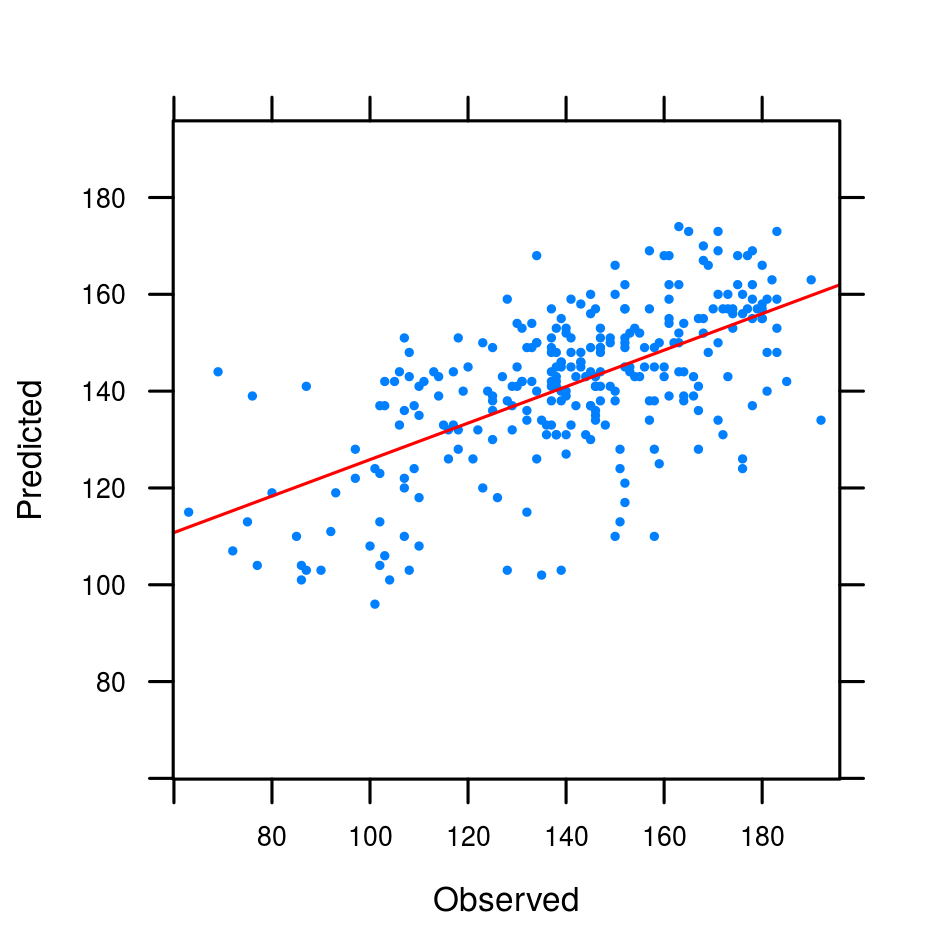
\includegraphics[width = 90mm, draft = true]{fig/chap07-random-forest-fit}
 \end{minipage}
 \begin{minipage}{90mm}
  \centering
  \subcaption{}
  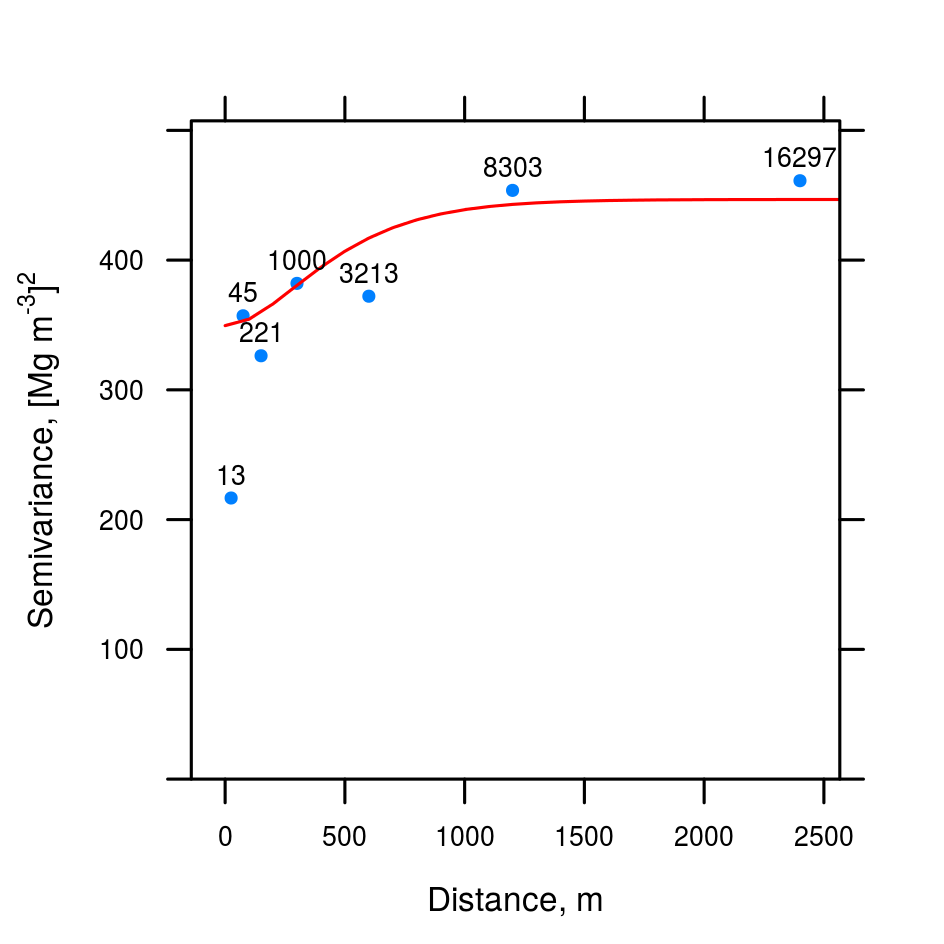
\includegraphics[width = 90mm]{fig/chap07-bude-vario}
 \end{minipage}
 \caption[(Non)Linear mixed model fitted to the soil bulk density data.]{(Non)Linear mixed model fitted to the 
 soil bulk density data (BUDE, \si{\mega\gram\per\cubic\metre}) measured at $n = 282$ calibration locations. 
 The top panel shows the relation between out-of-bag random regression forest predictions and BUDE, here
 representing the deterministic component $m(\boldsymbol{s})$. The bottom panel shows the REML fit of the 
 variogram model (red line) to BUDE, i.e. the stochastic component $e(\boldsymbol{s})$. Exponentially spaced
 lag-distance classes are used to depict the sample variogram (blue dots) along with the number of point-pairs
 in each variogram lag-distance class.}
 \label{fig:chap07-bude-vario}
\end{figure}

With the random regression forest and the LMM at hand, we produced $\mathcal{R} = 1000$ equiprobable 
realizations of an isotropic Gaussian random field of BUDE. Each realization is constituted of a collection of 
BUDE values at a fine grid of \num{\sim800000} regularly spaced (\SI{5}{\metre}) points covering the entire 
study area. Because we used \emph{unconditional} Gaussian simulation -- a simulation that is only 
\emph{globally} conditioned to the histogram (and variogram) of the data observed at the calibration locations 
\cite{Goovaerts1997} -- and a large number of realizations, we expect to find at any point of the simulation 
grid, over the $\mathcal{R} = 1000$ realizations, the whole set of possible BUDE values (i.e. the global 
histogram). Thus, the variance -- our uncertainty -- is the same everywhere. This is in contrast with 
\emph{conditional} Gaussian simulation -- a simulation that is \emph{locally} conditioned to the data observed 
at the calibration locations --, which serves the purposes of honouring the data at the calibration locations, 
thus reducing the variance of the output realizations \cite{Goovaerts1997}. In our study, \emph{conditional} 
Gaussian simulation is inappropriate as a model of uncertainty because the sampling algorithms that we evaluate 
are designed to situations where we know very little, everywhere, about the spatial structure of the soil data 
generating process.

Unconditional simulation algorithms approximate the globally conditioned distribution of a soil variable at a 
given point using neighbouring simulated values as local conditioning information \cite{Goovaerts1997}: the 
larger the neighbourhood, the better the approximation. A sensible criteria to select the nearest simulated 
values is the practical range of the variogram model \cite{Pebesma2004}. However, as the simulation proceeds, 
the number of simulated values within this neighbourhood becomes computationally prohibitive 
\cite{WebsterEtAl2007}. Thus, we chose to use a fixed maximum number of simulated values $n_{max} = 100$ 
within the practical range of the variogram model that are closest to the point being simulated. Last, but not 
least, sequential simulations algorithms speed up computations by using the same random path in all 
simulations, allowing it to reuse the \q{expensive results}: neighbourhood selection and solution to the 
kriging equations \cite{Pebesma2004}. We believe that following the same random path to generate each of the 
$\mathcal{R} = 1000$ realizations can introduce a structural component in the approximation errors. To avoid 
that, simulations were carried out using five different seeds for the pseudo-random number generators.

\subsection{Sampling and Model Calibration}

We compare $\mathcal{A} = 4$ sampling algorithms (CORR, DIST, ACDC, and CLHS) and $\mathcal{N} = 3$ sample 
sizes $n = (100, 200, 400)$. These sample sizes correspond to the moderately high inspection density (1 sample 
point per 20, 10, and \SI{5}{\hectare}, respectively) recommended for the production of soil maps published at 
a \scale{25000} \cite{Rossiter, 2000}.

We then sampled from each realization using the optimized spatial sample configurations. Because we wanted to 
check the effect of the sample size, each algorithms was run using $\mathcal{N} = 3$ sample sizes of $n = 
(100, 200, 400)$, which amounts to $\mathcal{D} = 3000}$ calibration datasets for each algorithm. Each 
calibration dataset was used to calibrate a random regression forest using the same covariates as used in 
simulating the fields.

\subsection{Evaluation of Sampling Algorithms}

The influence of sampling design and sample size on the spatial prediction accuracy will be assessed using 
$n = 1000$ validation points probabilistically selected from 500 quasi-equal-area compact geographic strata. 
Geographic stratification was obtained using the \textit{k}-means algorithm as implemented in the 
\Rpackage{spcosa} \cite{WalvoortEtAl2010}. Each strata has $n = 2$ randomly selected validation points. The 
algorithm was run using three different seeds for the pseudo-random number generator, the resulting 
stratification with the minimum objective value being selected.

We plan to use the realization-wise mean error (ME) and mean squared error (MSE) at the probabilistically 
validation points to evaluate the sampling designs. The ME will show the effect of the sampling design 
on the accuracy of the predictions, while the MSE will indicate how the sampling design influenced the 
calibration of the variogram model. As such, we can use the mean ratio of (empirical and theoretical) squared 
errors (MRSE) to see how good our estimate of the prediction errors are. The median of the ratio of squared 
errors (MedRSE) will also be computed because this ratio has a strong positive skew resulting that when there 
are have a few positive outliers of the ratio, the mean will be larger than 1 \cite{Lark2000a}. When the errors 
have normal distribution, the ratio has a chi-square distribution with 1 degree of freedom. So the median of 
the ratio then should be 0.455. A fifth measure that we plan to use is the amount of variance explained (AVE) 
by both the spatial trend and variogram model separately. At the end, we will aggregate these measures over the 
$\mathcal{R} = 1000$ realizations using box-and-whisker plots so that we can check visually how one sampling 
design compares to another.

\section{RESULTS AND DISCUSSION}

\begin{figure}[!ht]
 \centering
 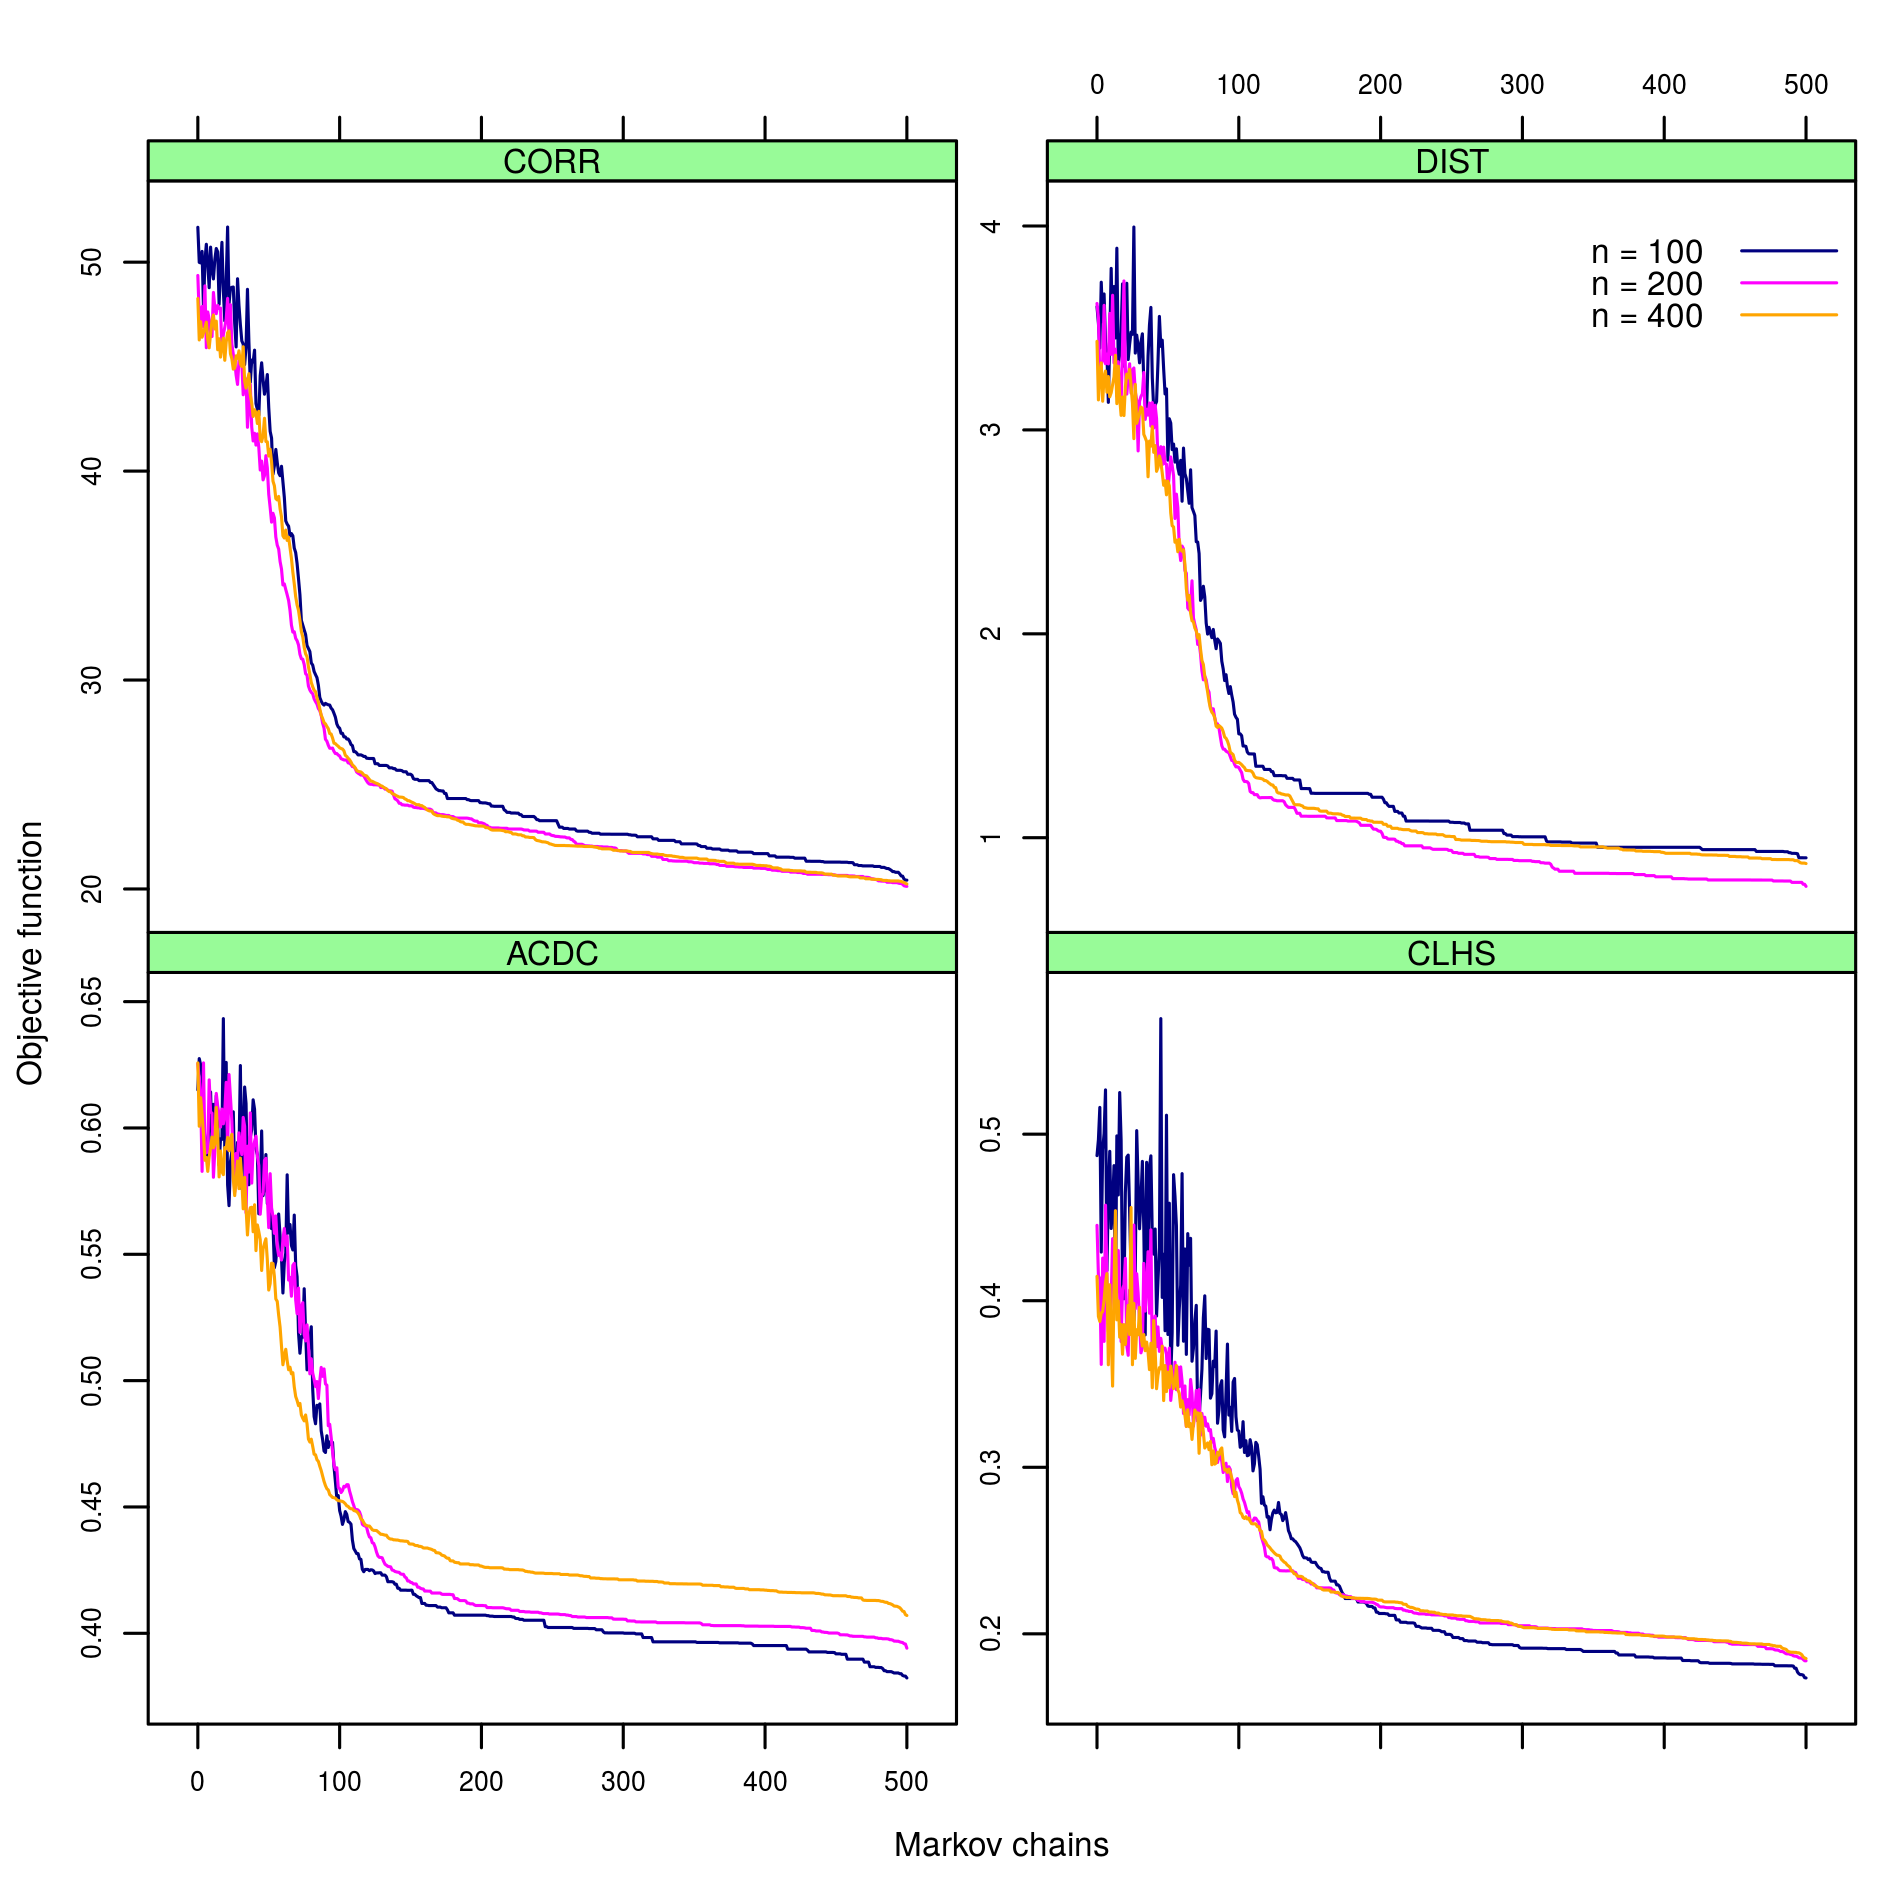
\includegraphics[width=\textwidth]{fig/chap07-energy_corr_dist_acdc_clhs}
 \caption[Objective function values during the optimization of three sample configurations using four sampling 
 algorithms.]{Objective function values during the optimization of sample configurations of size 
 $n = (100, 200, 400$) using sampling algorithms CORR, DIST, ACDC, and CLHS against the number of Markov 
 chains of length $n$.}
 \label{fig:chap07-energy-all}
\end{figure}

\begin{figure}[!ht]
 \centering
 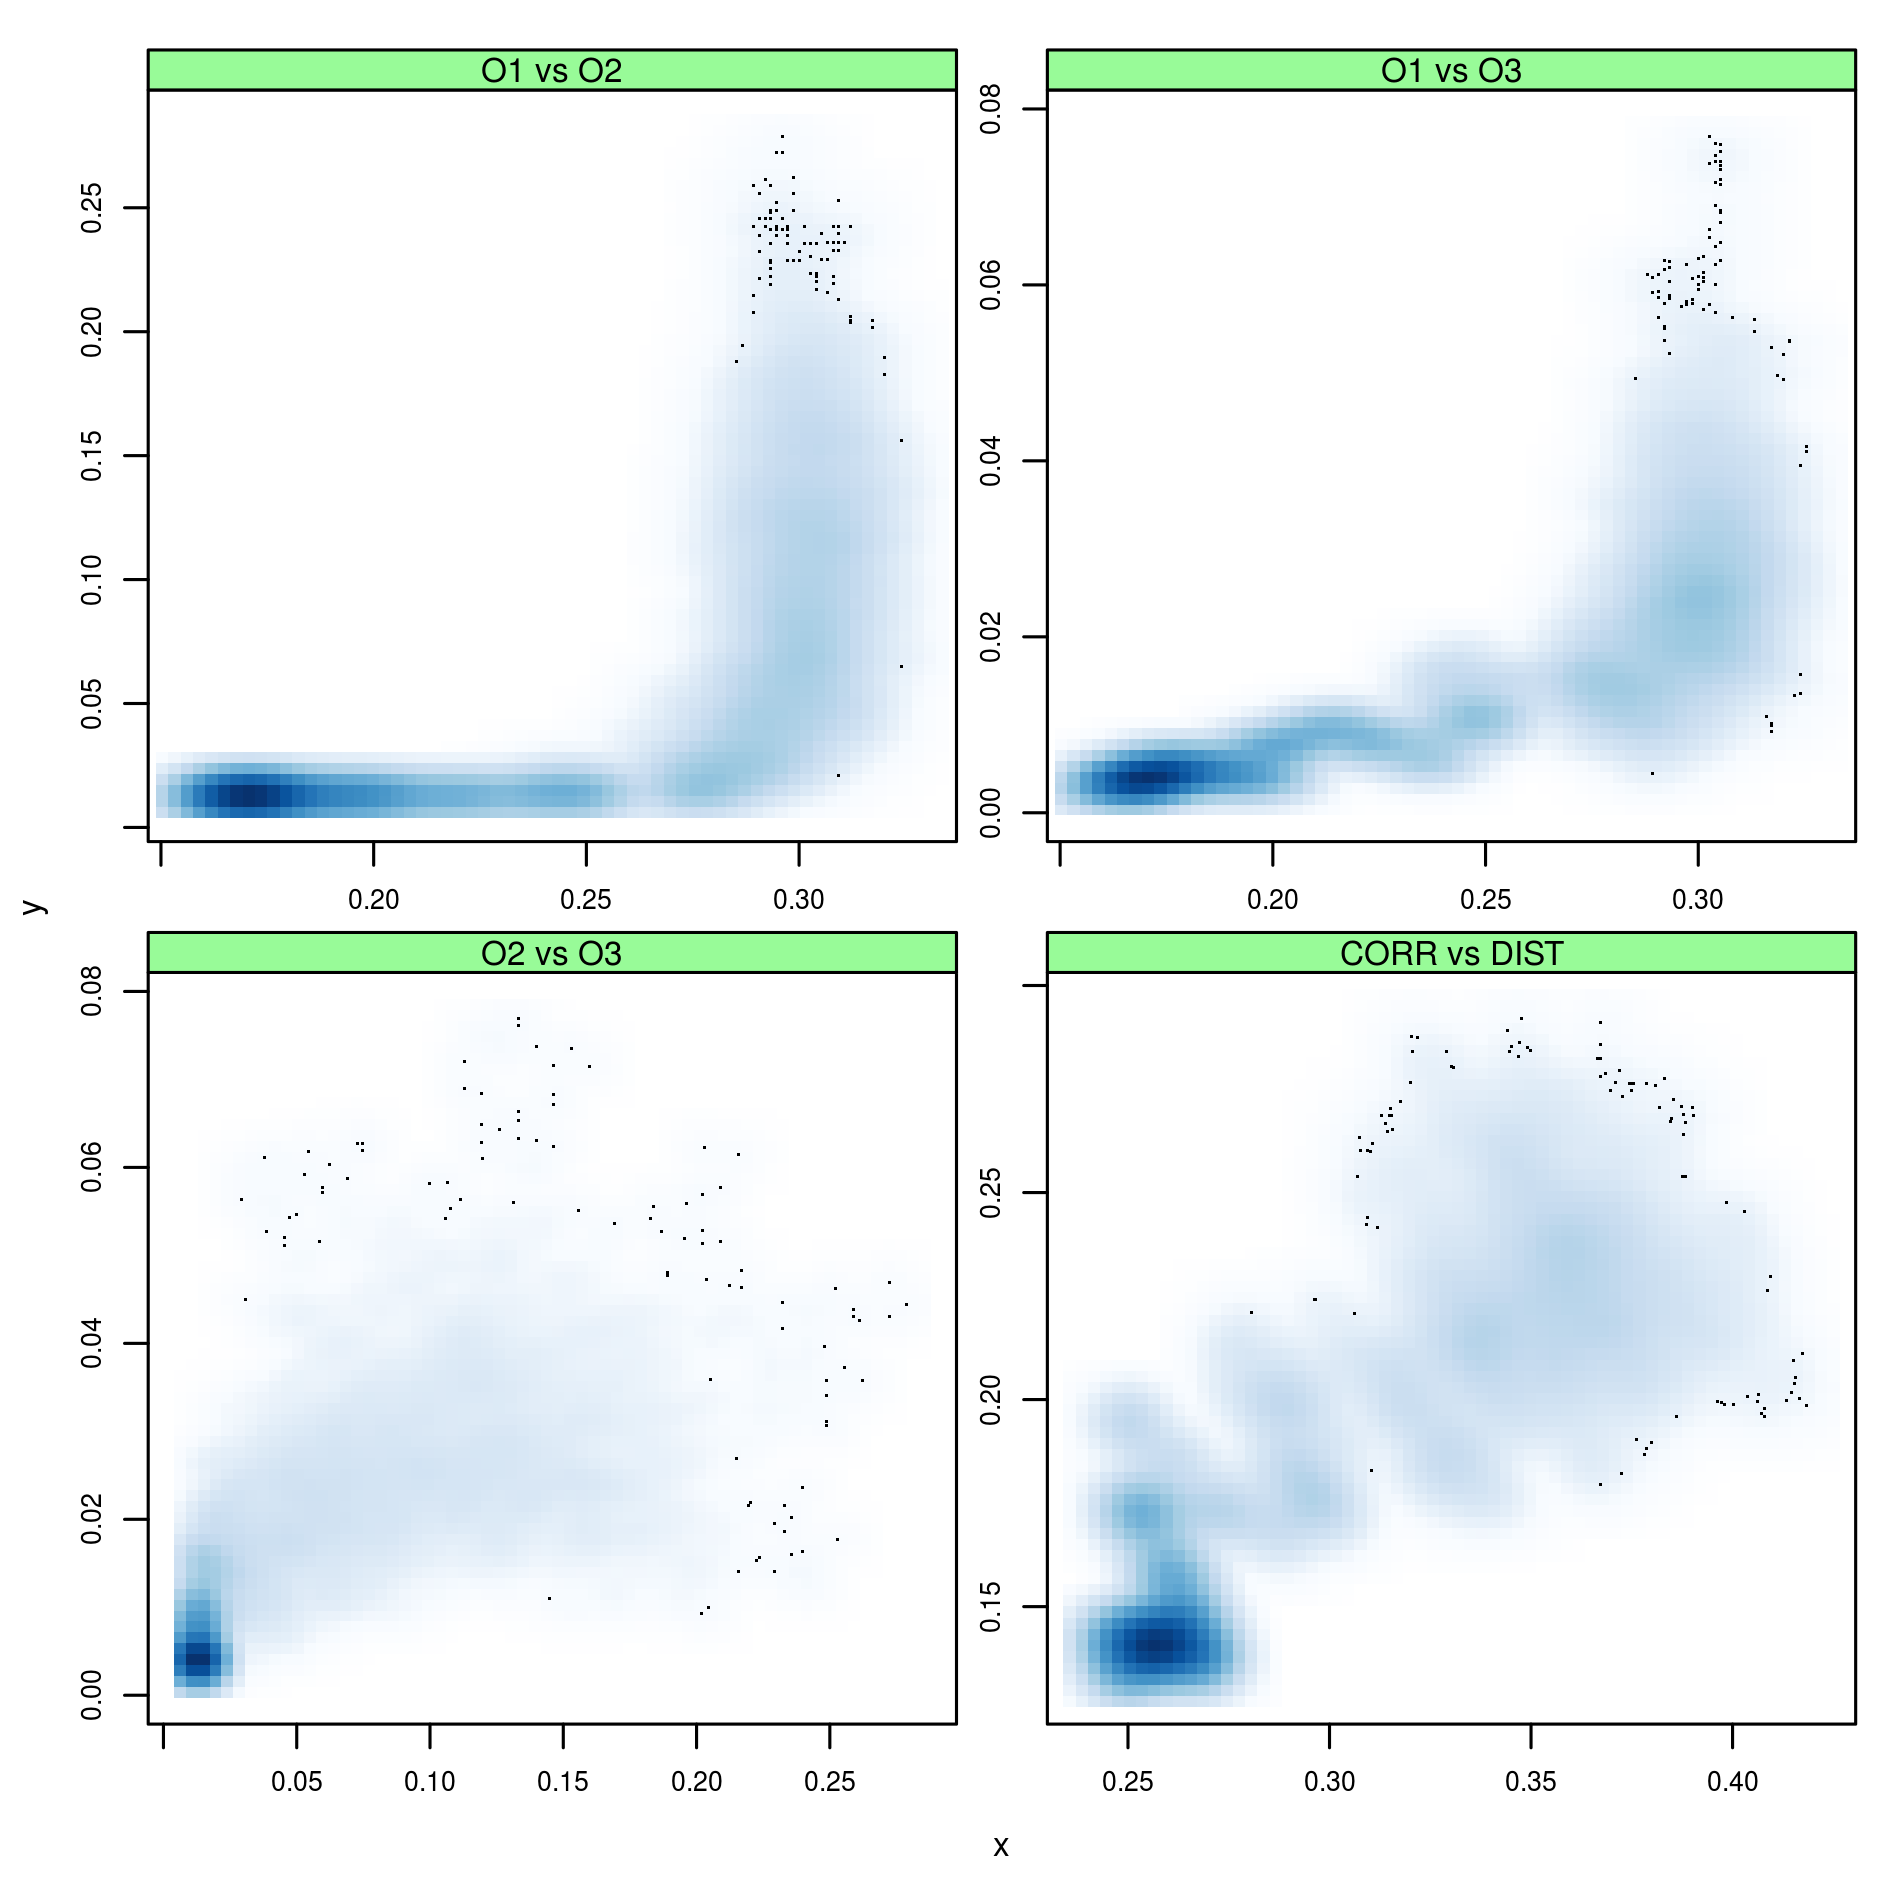
\includegraphics[width=\textwidth]{fig/chap07-energy_acdc_clhs}
 \caption[Region of the feasible objective space explored by pairs of objective functions that compose CLHS 
 and ACDC.]{Region of the feasible objective space $\mathcal{Z}$ explored by pairs of objective functions (x 
 vs  y) that compose CLHS ($\mathcal{O}_1$, $\mathcal{O}_2$, and $\mathcal{O}_3$) and ACDC (CORR and DIST)  
 during the optimization of a sample configuration of size $n = 100$ using $n_{\text{chains}} = 500$ Markov 
 chains of length $n$.}
 \label{fig:chap07-energy-acdc-clhs}
\end{figure}

\begin{figure}[!ht]
 \centering
 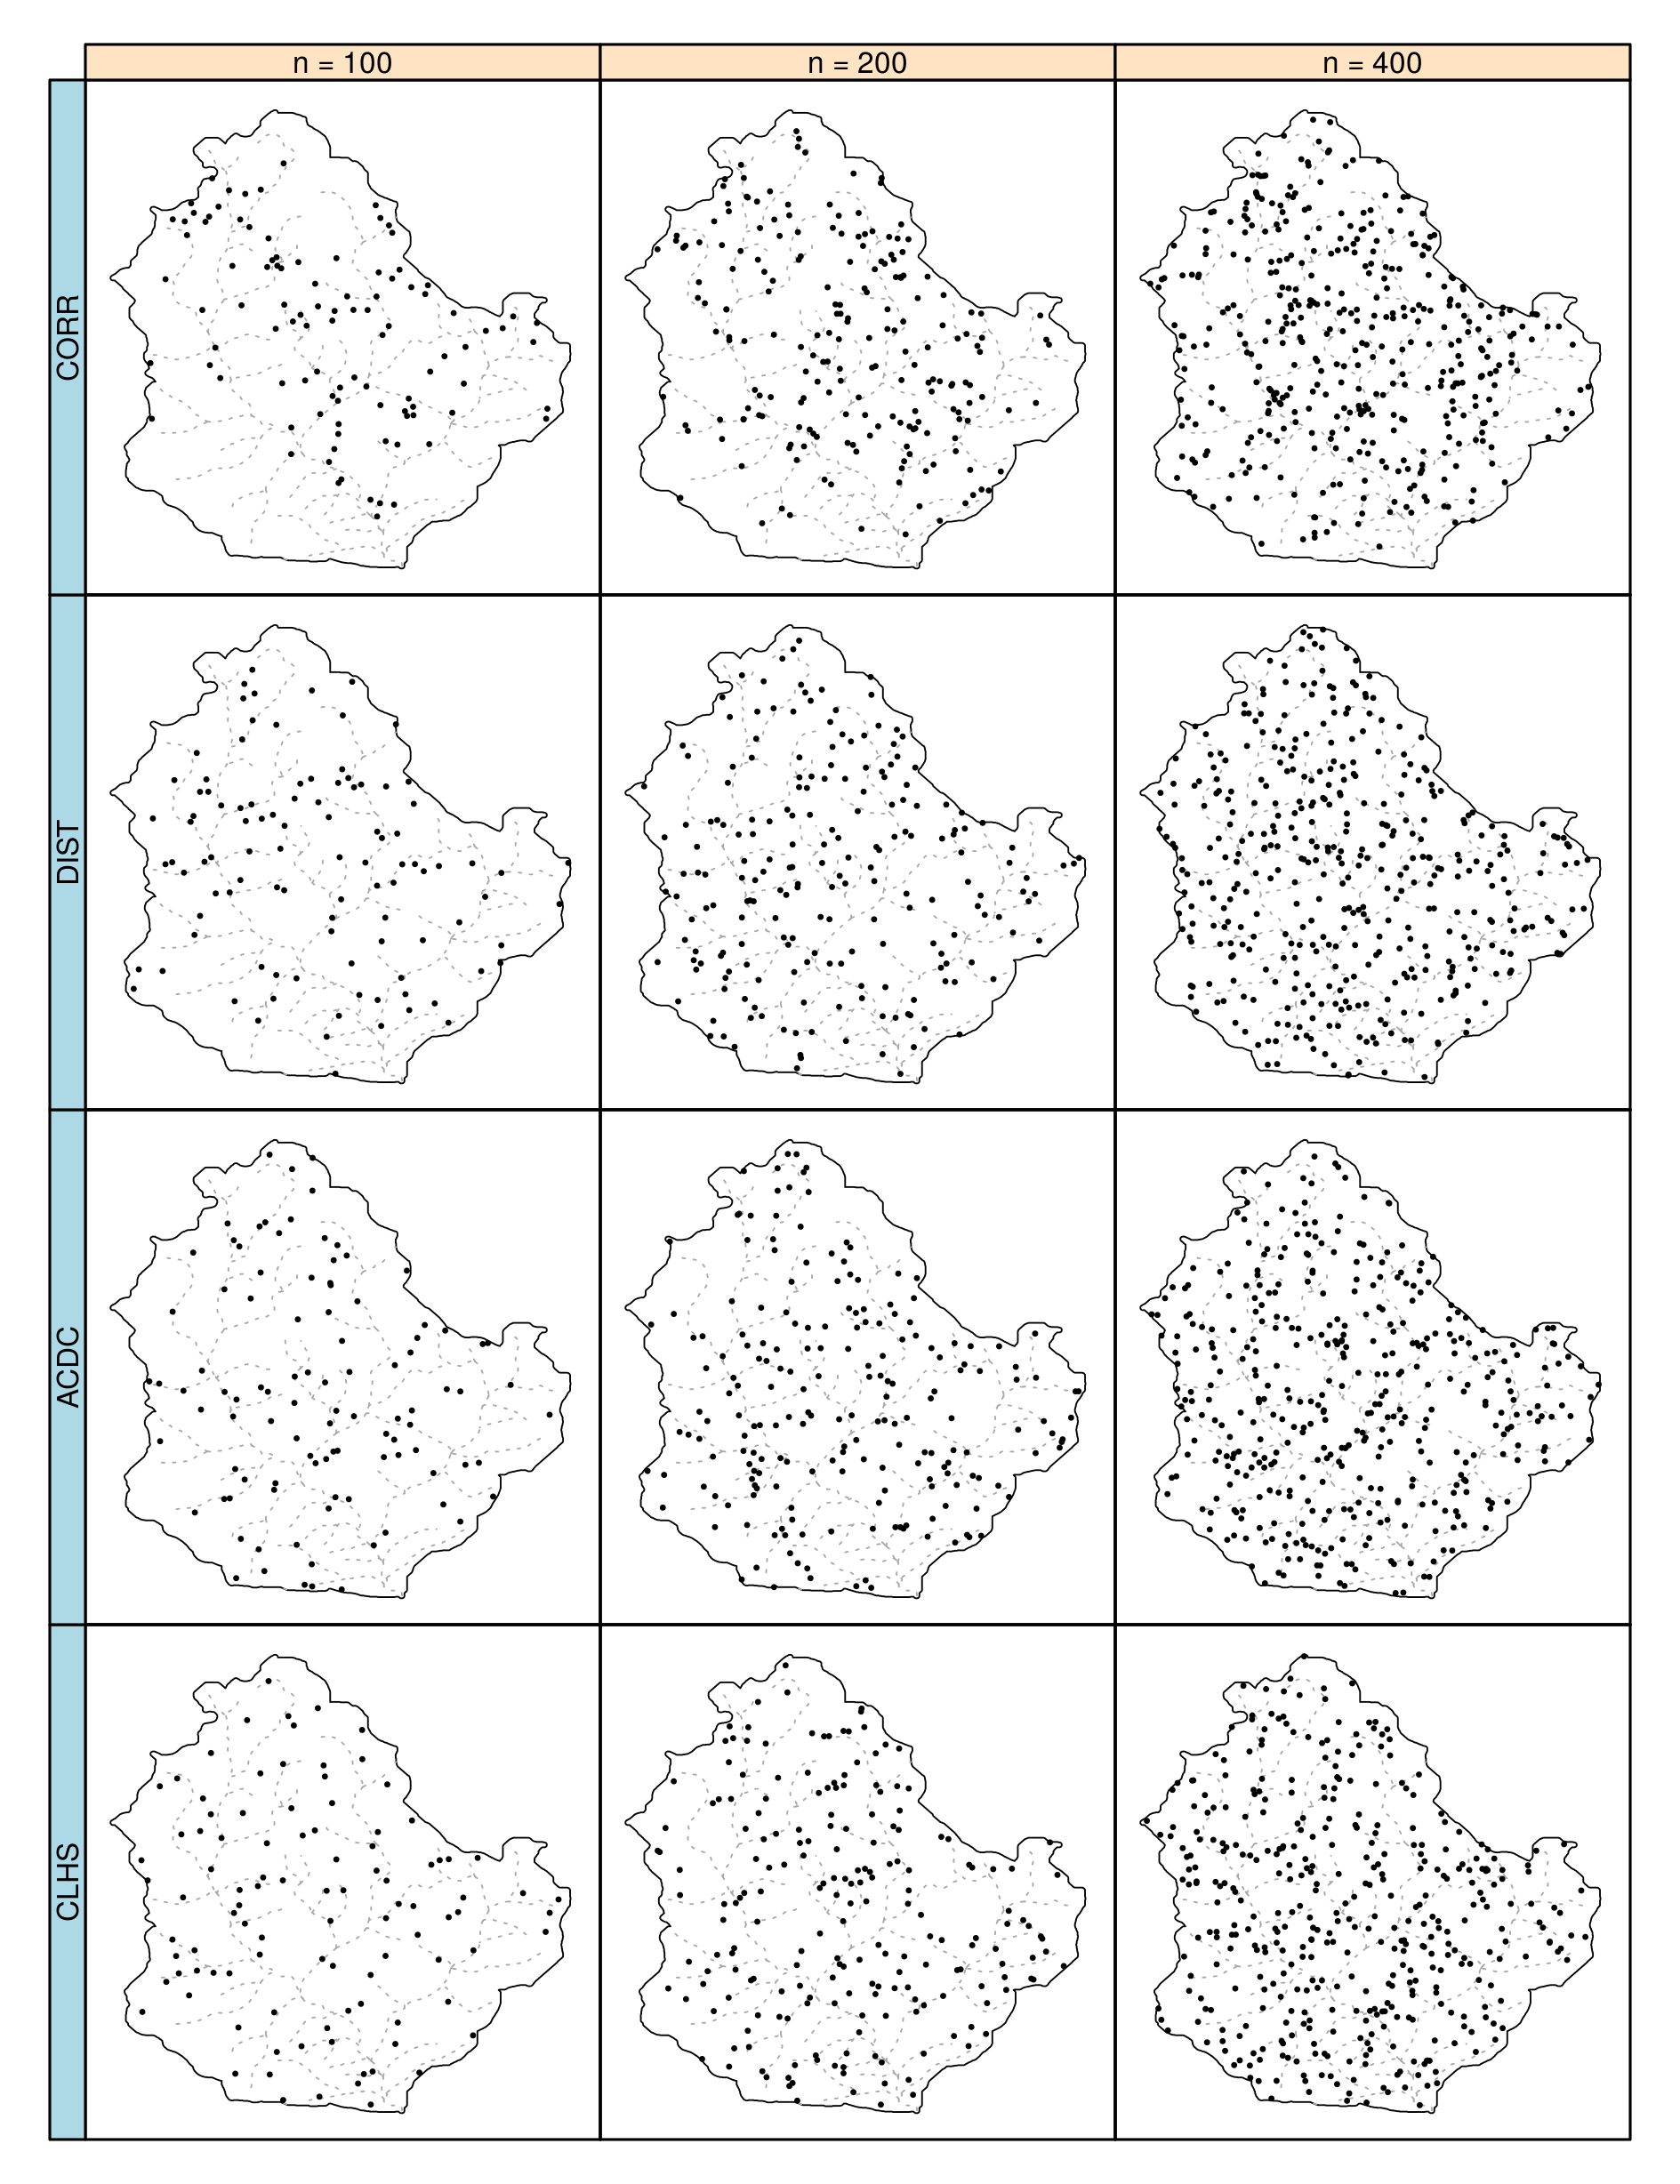
\includegraphics[width=\textwidth]{fig/chap07-points_corr_dist_acdc_clhs}
 \caption[Sample configurations optimized using four sampling algorithms.]{Sample configurations of size 
 $n = (100, 200, 400)$ optimized using sampling algorithms CORR, DIST,  ACDC, and CLHS superimposing the
 drainage network.}
 \label{fig:chap07-points}
\end{figure}

\section{FINAL CONSIDERATIONS}


